\documentclass{article}

% NeurIPS 2026 preprint template.
\PassOptionsToPackage{numbers,compress}{natbib}
\PassOptionsToPackage{hidelinks}{hyperref}
\usepackage[preprint]{neurips_2026}

\usepackage[utf8]{inputenc}
\usepackage[T1]{fontenc}
\usepackage{microtype}
\usepackage{amsmath,amssymb}
\usepackage{booktabs}
\usepackage{enumitem}
\usepackage{graphicx}
\usepackage{tabularx}
\usepackage{multirow}
\usepackage{xcolor}
\usepackage{hyperref}

\title{Compression Safety in Biomedical Vision Models\\
Clinical Evaluation of Pruning, Quantization, and Distillation on HAM10000}

\author{%
  Abdulla Alfalasi \\
  ML8505 --- Tiny Machine Learning \\
  Mohamed Bin Zayed University of AI \\
  \And
  Mohammed Ibrahim \\
  ML8505 --- Tiny Machine Learning \\
  Mohamed Bin Zayed University of AI \\
}
\date{}

\newcommand{\mel}{\ensuremath{\textit{mel}}}
\newcommand{\bcc}{\ensuremath{\textit{bcc}}}
\newcommand{\akiec}{\ensuremath{\textit{akiec}}}
\newcommand{\nv}{\ensuremath{\textit{nv}}}
\newcommand{\DCR}{\ensuremath{\mathrm{DCR}}}

\begin{document}
\maketitle

\begin{abstract}
Compression studies for medical imaging usually report a single accuracy number. That number hides what clinicians need to know: whether the rare dangerous classes are still detected, and whether the model's confidence can still be trusted. We study this for skin lesion classification on HAM10000 with DeiT-Tiny and DeiT-Small.

We compare four pruning rules (magnitude, Wanda, Taylor, random), sensitivity-guided non-uniform sparsity, INT8 post-training quantization, and knowledge distillation. In addition to balanced accuracy, melanoma AUROC, ECE, and model size, we report a Dangerous-Class Degradation Ratio (\DCR{}), which measures how much more performance drops on the three dangerous lesion classes (melanoma, basal cell carcinoma, and actinic keratosis) than on the safer classes.

We find the following. (i) Magnitude pruning is the least safe baseline. It has the highest \DCR{} and loses dangerous-class recall first. (ii) Taylor pruning at 50\% sparsity gives the best clinical tradeoff, with strong melanoma discrimination and low calibration error. The ordering holds across the 20--70\% sweep, and a per-layer gradient-flow analysis explains it. (iii) INT8 quantization preserves dense-model behavior and cuts size by 3.8$\times$. (iv) Non-uniform sparsity can rescue Wanda when recall matters, but it shifts the error profile and needs calibration-aware validation. Distillation does not improve the dense DeiT-Tiny student on average and makes it less robust to pruning.

We contribute a deployment-oriented evaluation protocol and a set of recommendations for biomedical vision models. We do not propose a new compression technique.
\end{abstract}

\section{Introduction}
Biomedical vision models are most useful where deployment is most constrained: dermatology screening in low-connectivity clinics, point-of-care triage, and mobile or edge-assisted second reads. Memory footprint, latency, and privacy all matter in these settings, so compression is often what makes a model deployable at all.

Conventional evaluation hides the failure mode that matters most clinically. HAM10000 is strongly imbalanced: \nv{} dominates the dataset, while melanoma, basal cell carcinoma, and actinic keratosis are much rarer. A compressed model can keep its balanced accuracy while its performance on the classes clinicians care most about degrades, and a paper that reports only one aggregate number can present this degradation as progress.

We ask a practical question: when a medical Vision Transformer is compressed, which choices preserve diagnostic safety, and which only preserve headline metrics? We treat this as a deployment problem. Our contribution is an evaluation protocol that exposes class-asymmetric failure, together with recommendations for biomedical teams that want to compress models without taking on avoidable risk.

Our main contributions are:
\begin{itemize}[leftmargin=*,itemsep=2pt,topsep=2pt]
\item We introduce \DCR{}, a compact safety metric that measures whether compression harms dangerous lesions more than safer ones.
\item We run lesion-grouped, multi-seed pruning comparisons on DeiT-Tiny and DeiT-Small across the full 20--70\% sparsity sweep. Magnitude is the least safe baseline and Taylor is the strongest sparse default.
\item We measure attention overlap with lesion masks and show that Wanda's failure happens downstream of attention; Wanda still localizes lesions.
\item We add a gradient-flow probe showing that magnitude pruning concentrates on high-gradient layers while Taylor avoids them, and we rule out the simpler activation-concentration hypothesis.
\item We run the deployment experiments that biomedical integrators ask about: non-uniform sparsity, INT8 stacking, knowledge distillation, recovery fine-tuning, calibration-size ablation, and a MobileNetV2 baseline.
\item We turn these results into practical recommendations: use lesion-grouped splits, report AUROC and calibration alongside sensitivity, start with INT8, use Taylor rather than magnitude when sparsity is required, and treat every evaluated pipeline as academic-only unless it clears the conservative clinical thresholds.
\end{itemize}

\section{Related Work}
\paragraph{Pruning and sparsity.}
Magnitude pruning \cite{han2015deep} remains the standard baseline because it is simple and cheap to compute. Taylor scoring \cite{molchanov2017taylor} accounts for the loss gradient, which makes it sensitive to the task. Wanda \cite{sun2023wanda} carries activation-aware pruning from language models over to vision by combining weight magnitude with activation norm. Biomedical pruning studies usually evaluate aggregate accuracy, which says little about class-specific safety.

\paragraph{Quantization and distillation.}
INT8 post-training quantization is a mature deployment technique with a well-understood efficiency tradeoff \cite{jacob2018quantization,gholami2021survey}. Knowledge distillation \cite{hinton2015distillation} and DeiT-style training \cite{touvron2021deit} can improve dense model quality, but it is not obvious that a better dense student is also more robust to pruning.

\paragraph{Medical evaluation.}
Recent work on medical pruning and explainability focuses on fairness, interpretability, or sparsity quality \cite{paxton2025,yu2023xpruner}. We ask a narrower deployment question: does compression move the diagnostic operating point in ways that affect lesion triage, referral, and screening?

\paragraph{Attention analysis.}
Attention rollout and attention-flow metrics \cite{abnar2020attention} are often used qualitatively. We use them more conservatively, to check whether pruning destroys lesion localization or whether the failure happens later in the pipeline.

\section{Method}
\paragraph{Dataset and splits.}
We use HAM10000 \cite{tschandl2018ham10000}, which contains 10{,}015 dermoscopic images across seven classes: \akiec{}, \bcc{}, \textit{bkl}, \textit{df}, \mel{}, \nv{}, and \textit{vasc}. We build splits with lesion-grouped \texttt{GroupShuffleSplit} on \texttt{lesion\_id}, so each lesion goes entirely to train or to validation. Image-level splitting would leak lesion-specific cues across the split and inflate the reported metrics.

\paragraph{Models and compression.}
We fine-tune DeiT-Tiny and DeiT-Small from \texttt{timm}. DeiT-Small is also the teacher in the distillation experiment. We compare four one-shot pruning criteria at several sparsities: magnitude, Wanda, Taylor, and random. We also evaluate sensitivity-guided non-uniform sparsity, INT8 post-training quantization, knowledge distillation as a pre-treatment, post-pruning recovery fine-tuning, a calibration-size ablation, and a MobileNetV2 baseline.

\paragraph{Clinical metrics.}
We report balanced accuracy, per-class sensitivity, melanoma AUROC, macro AUROC, ECE, model size, and latency. We also define the dangerous-class degradation ratio:
\begin{equation}
\DCR = \frac{\frac{1}{|\mathcal{D}|}\sum_{c \in \mathcal{D}}\left[\mathrm{Sens}^{\text{dense}}_c - \mathrm{Sens}^{\text{comp}}_c\right]}{\frac{1}{|\mathcal{S}|}\sum_{c \in \mathcal{S}}\left[\mathrm{Sens}^{\text{dense}}_c - \mathrm{Sens}^{\text{comp}}_c\right]},
\end{equation}
where $\mathcal{D}=\{\mel,\bcc,\akiec\}$ and $\mathcal{S}=\{\nv,\textit{bkl},\textit{df},\textit{vasc}\}$. Values above 1 mean compression hurts dangerous classes more than safer ones.

\paragraph{Protocol.}
Headline pruning results are mean $\pm$ standard deviation across the available seeds. Direct method comparisons use paired tests on matched seeds. The main pruning comparison is at 50\% sparsity, the most informative tradeoff point for biomedical deployment.

\paragraph{Clinical regime tagging.}
We map each aggregated run to one of four conservative clinical regimes: \texttt{triage\_screen}, \texttt{specialist\_referral}, \texttt{primary\_diagnosis}, or \texttt{academic\_only}. The thresholds come from the log companion files and are deliberately strict. Every evaluated pipeline in this study is tagged \texttt{academic\_only}, which is the expected outcome for a study that measures compression safety and makes no claim of clinical readiness.

\section{Results}

\subsection{Pruning criteria at 50\% sparsity}
Table~\ref{tab:headline} summarizes the main pruning comparison. Magnitude is the least safe baseline, Taylor gives the strongest sparse tradeoff, and Wanda has the worst calibration even when it preserves some recall.

\begin{table*}[t]
\centering
\small
\caption{Headline pruning results at 50\% sparsity. Beyond average performance, the question is which method avoids preferentially forgetting dangerous classes. Dense baselines are shown for reference.}
\label{tab:headline}
\resizebox{\textwidth}{!}{%
\begin{tabular}{llccccccc}
\toprule
Model & Criterion & Bal.\ Acc. & Mel.\ Sens. & Mel.\ AUROC & Macro AUROC & ECE & \DCR & Spec@90Sens \\
\midrule
\multirow{5}{*}{DeiT-Small}
 & Dense       & $0.914 \pm 0.032$ & $0.896 \pm 0.030$ & $0.964 \pm 0.010$ & $0.986 \pm 0.008$ & $0.017 \pm 0.009$ & --- & $0.905 \pm 0.031$ \\
 & Magnitude   & $0.789 \pm 0.026$ & $0.571 \pm 0.052$ & $0.881 \pm 0.018$ & $0.959 \pm 0.007$ & $0.035 \pm 0.008$ & $1.89 \pm 0.42$ & $0.663 \pm 0.029$ \\
 & Wanda       & $0.612 \pm 0.018$ & $0.541 \pm 0.042$ & $0.837 \pm 0.018$ & $0.923 \pm 0.006$ & $0.099 \pm 0.005$ & $0.77 \pm 0.09$ & $0.568 \pm 0.044$ \\
 & Taylor      & $0.770 \pm 0.032$ & $0.843 \pm 0.031$ & $0.931 \pm 0.012$ & $0.973 \pm 0.006$ & $0.031 \pm 0.007$ & $0.95 \pm 0.26$ & $0.795 \pm 0.042$ \\
 & Random      & $0.133 \pm 0.011$ & $0.000 \pm 0.000$ & $0.523 \pm 0.049$ & $0.537 \pm 0.032$ & $0.249 \pm 0.125$ & $0.99 \pm 0.36$ & $0.170 \pm 0.028$ \\
\midrule
\multirow{5}{*}{DeiT-Tiny}
 & Dense       & $0.906 \pm 0.035$ & $0.845 \pm 0.038$ & $0.951 \pm 0.011$ & $0.984 \pm 0.005$ & $0.025 \pm 0.009$ & --- & $0.869 \pm 0.035$ \\
 & Magnitude   & $0.758 \pm 0.038$ & $0.518 \pm 0.048$ & $0.895 \pm 0.014$ & $0.960 \pm 0.006$ & $0.049 \pm 0.005$ & $3.83 \pm 1.66$ & $0.695 \pm 0.044$ \\
 & Wanda       & $0.338 \pm 0.010$ & $0.934 \pm 0.019$ & $0.799 \pm 0.024$ & $0.823 \pm 0.010$ & $0.118 \pm 0.006$ & $0.63 \pm 0.06$ & $0.558 \pm 0.045$ \\
 & Taylor      & $0.585 \pm 0.016$ & $0.814 \pm 0.121$ & $0.868 \pm 0.027$ & $0.942 \pm 0.007$ & $0.039 \pm 0.010$ & $0.99 \pm 0.18$ & $0.630 \pm 0.053$ \\
 & Random      & $0.140 \pm 0.006$ & $0.964 \pm 0.089$ & $0.482 \pm 0.080$ & $0.540 \pm 0.025$ & $0.148 \pm 0.038$ & $0.67 \pm 0.05$ & $0.168 \pm 0.077$ \\
\bottomrule
\end{tabular}}
\end{table*}

The failure mode depends on the scoring rule. Magnitude has the highest \DCR{} on both backbones ($1.89$ on DeiT-Small, $3.83$ on DeiT-Tiny), and on DeiT-Tiny it also has the lowest melanoma sensitivity of any non-random criterion. Wanda preserves some dangerous-class recall on DeiT-Small, but its calibration is much worse and its discrimination is markedly weaker. Taylor is the only criterion that stays in the clinically useful part of the tradeoff curve on both backbones.

\subsection{Full sparsity sweep and significance}
Table~\ref{tab:headline} shows only the 50\% point. The full 20--70\% sweep preserves the same ordering, although the shape of the failure changes with backbone and criterion. At 20\% sparsity, all three criteria stay close to dense on DeiT-Small: magnitude reaches $0.920$ balanced accuracy with $0.908$ melanoma sensitivity, Wanda reaches $0.915$ / $0.870$, and Taylor reaches $0.915$ / $0.885$. By 40\%, the two backbones begin to diverge. By 60--70\%, magnitude and Wanda have left the clinically useful frontier for different reasons, and Taylor is the only criterion that still keeps nontrivial discrimination on both backbones.

Paired tests show that the 50\% comparison is not a seed artifact. The Wanda vs.\ magnitude difference in balanced accuracy is highly significant on both backbones ($p < 10^{-15}$), but melanoma sensitivity moves in different directions. On DeiT-Small, magnitude slightly exceeds Wanda on melanoma sensitivity. On DeiT-Tiny, Wanda overshoots melanoma sensitivity by nearly $0.42$ while its balanced accuracy collapses. This is why we keep AUROC and ECE in the table: sensitivity alone would make the smaller backbone look safer than it is.

At 70\% sparsity, DeiT-Small magnitude and Wanda both lose melanoma sensitivity entirely, while Taylor still has balanced accuracy above $0.42$ and melanoma sensitivity above $0.36$. On DeiT-Tiny, Wanda reaches a melanoma sensitivity of $1.000$ at 70\%, but this is a threshold artifact: balanced accuracy is $0.143$ and ECE remains high. The full sweep leaves the ranking unchanged and shows how each criterion fails.

\begin{figure*}[t]
\centering
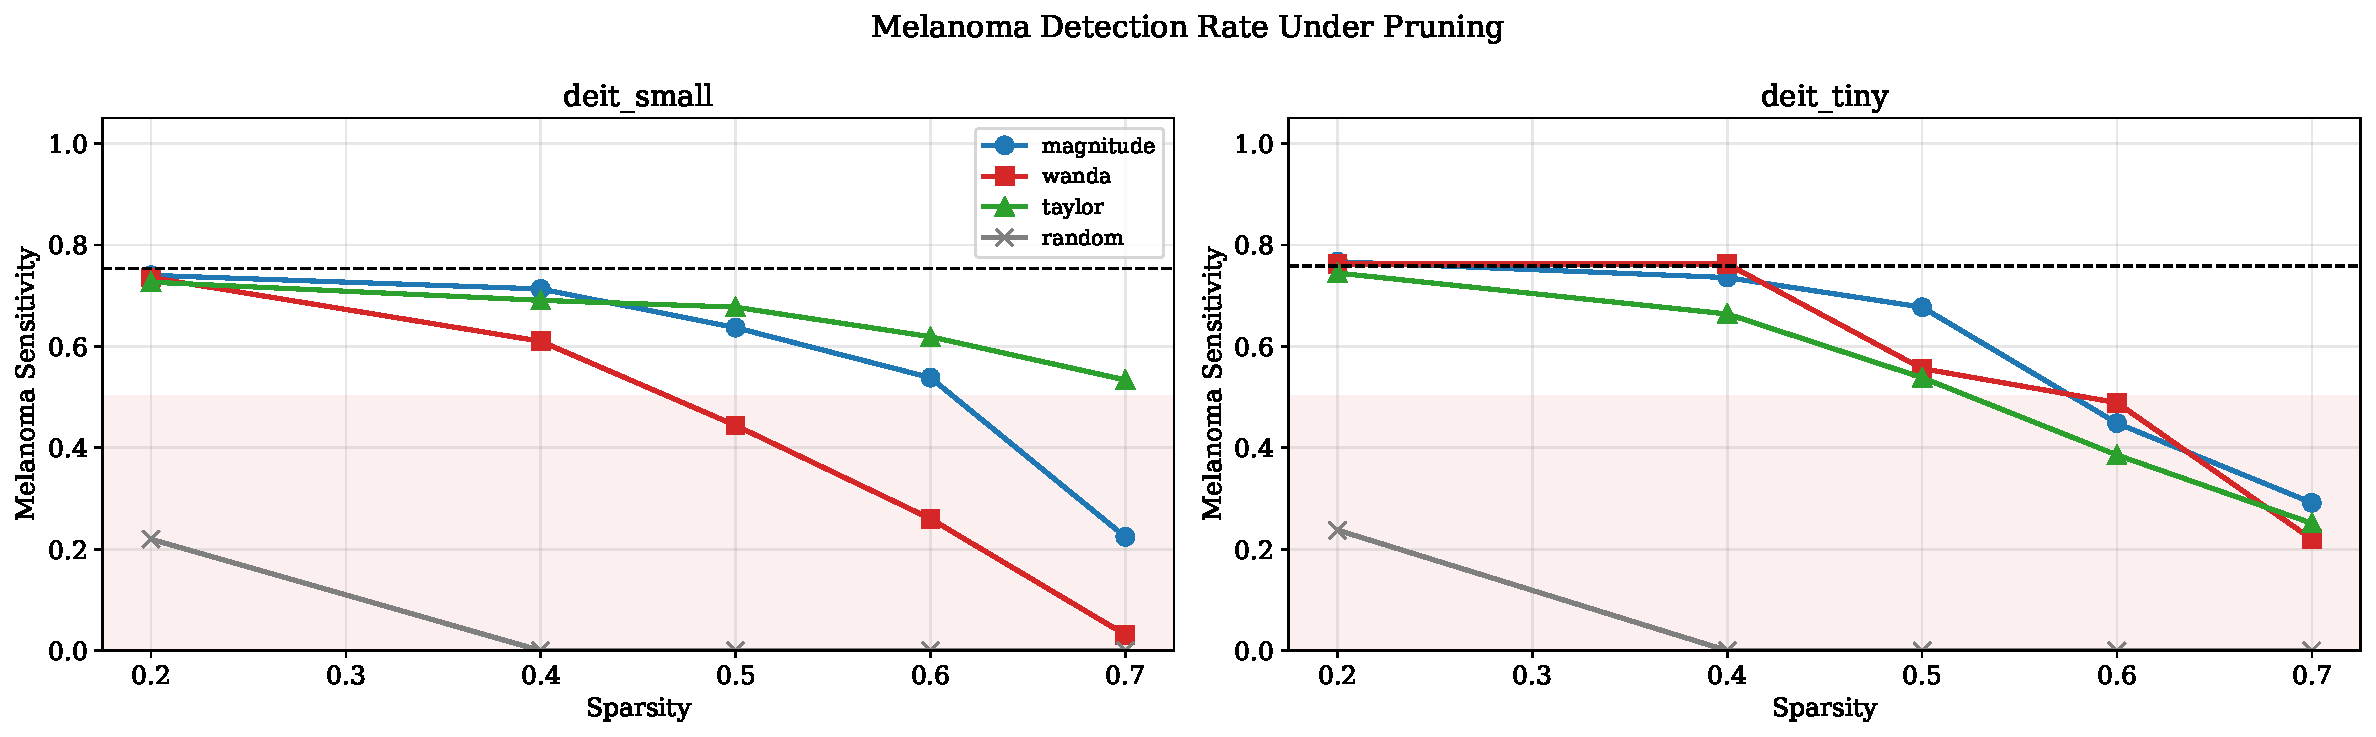
\includegraphics[width=0.49\textwidth]{../results/figures_local/fig1_melanoma_sensitivity.pdf}
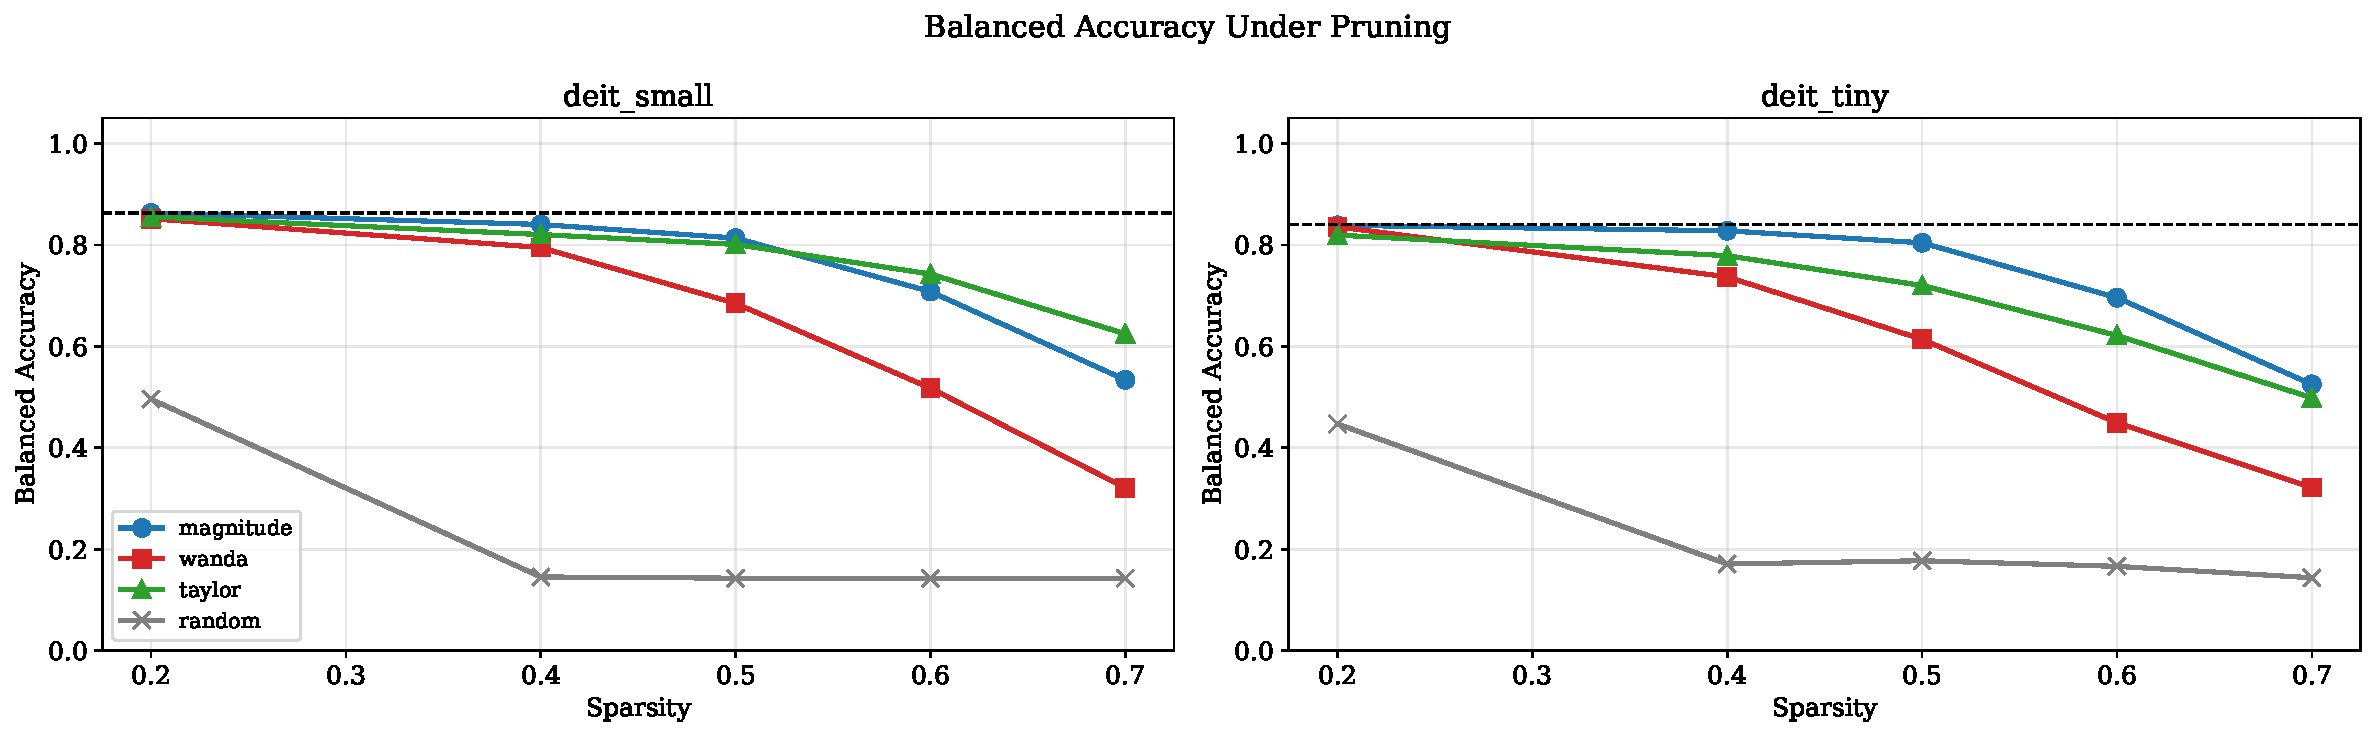
\includegraphics[width=0.49\textwidth]{../results/figures_local/fig2_balanced_accuracy.pdf}
\caption{Behavior across sparsity levels from the project's exploratory run. Melanoma sensitivity can rise while balanced accuracy collapses, so sensitivity alone is not a sufficient safety signal. Taylor has the most stable sparse frontier; Wanda's behavior depends strongly on model scale.}
\label{fig:sparsity_curves}
\end{figure*}

\subsection{Safety is not captured by sensitivity alone}
Figure~\ref{fig:sparsity_curves} is the main reason we report several metrics. On DeiT-Tiny, Wanda inflates melanoma sensitivity while balanced accuracy and AUROC collapse. This is a threshold shift, and a sensitivity-only report would mistake over-prediction for discrimination.

A screening model that over-calls melanoma looks safer in a sensitivity-only table, but the false-positive burden can make it useless in practice. AUROC and calibration separate genuine improvement from prediction collapse. Figure~\ref{fig:sens_vs_auroc} places every (backbone, criterion) point at 50\% sparsity in the sensitivity-AUROC plane. Wanda on DeiT-Tiny lands inside the shaded ``classifier collapse'' region (high sensitivity, low AUROC), while Taylor and the dense baselines stay in the clinically useful upper-right corner.

\begin{figure}[t]
\centering
\includegraphics[width=\linewidth]{../results/figures_personal/fig_mel_sens_vs_auroc.pdf}
\caption{Melanoma sensitivity versus melanoma AUROC at 50\% sparsity. The shaded region marks classifier collapse, where high sensitivity coexists with low discrimination. Wanda on DeiT-Tiny falls inside this region, so a sensitivity-only report would misread it as the safest configuration.}
\label{fig:sens_vs_auroc}
\end{figure}

\begin{figure}[t]
\centering
\includegraphics[width=\linewidth]{../results/figures_personal/fig_dcr_bars.pdf}
\caption{Dangerous-Class Degradation Ratio on the multi-seed personal aggregate. Magnitude degrades dangerous classes more than safer ones, and Wanda reverses the direction of the imbalance. Taylor stays closest to a balanced tradeoff.}
\label{fig:dcrbars}
\end{figure}

\subsection{Why the criteria behave differently}
Figure~\ref{fig:dcrbars} shows the safety asymmetry directly. Magnitude pruning is a dangerous default: its \DCR{} is above 1 on both backbones, so it degrades the classes that were already underrepresented during fine-tuning more than the common ones. Wanda preserves a subset of high-activation features, which does not guarantee better discrimination: in our results, its dangerous-class recall can look acceptable while calibration degrades sharply.

Taylor scoring uses the loss gradient, and in an imbalanced biomedical problem that gradient already carries class information. Taylor therefore tends to keep the decision-critical layers intact. Its advantage over magnitude comes from alignment with the task rather than from extra sophistication.

\begin{figure}[t]
\centering
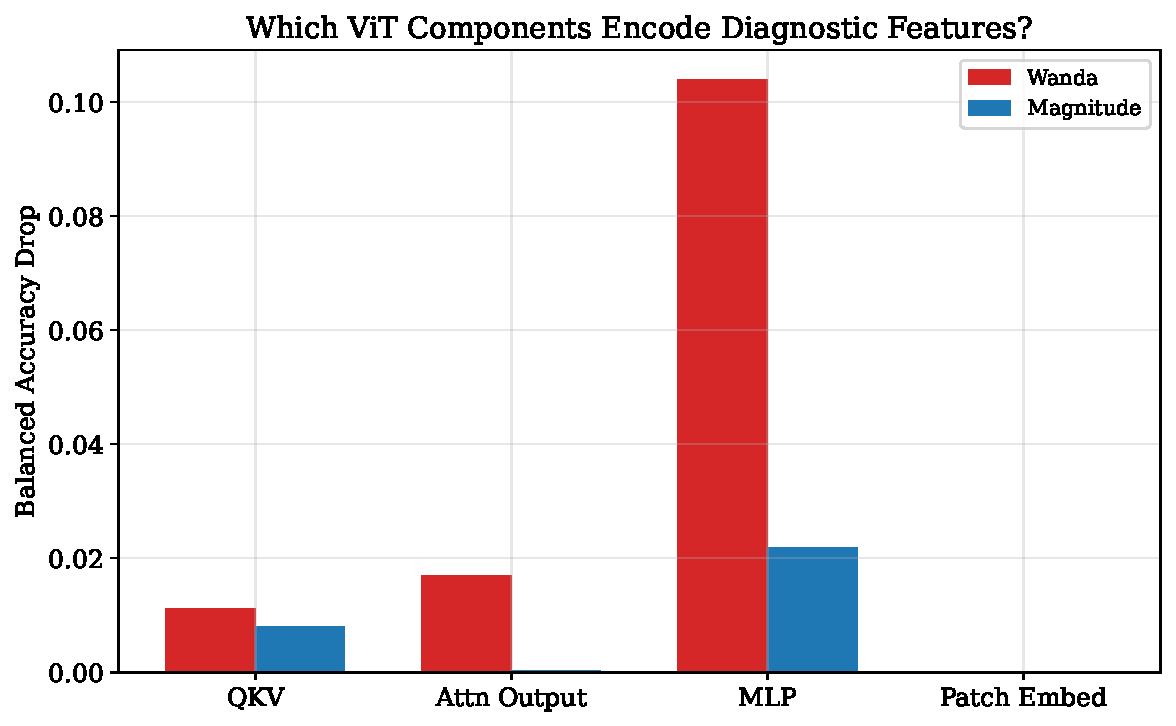
\includegraphics[width=\linewidth]{../results/figures_local/fig3_perlayer_bars.pdf}
\caption{Exploratory per-layer analysis from the local run. Bars show how much balanced accuracy each ViT component loses when pruned on its own. The MLP blocks are the main sensitivity hotspot, and patch embedding is comparatively stable. This supports the view that where sparsity is placed matters more than a single global score.}
\label{fig:perlayer}
\end{figure}

\paragraph{Mechanism.}
The per-layer analysis in Figure~\ref{fig:perlayer} indicates that the MLP blocks matter most for diagnostic behavior. This fits the broader result that which layers get pruned matters more than the parameter count or the name of the criterion.

We also tested an activation-outlier hypothesis: that Wanda succeeds or fails because it over-protects layers with unusually concentrated activations. The correlations in the project summary were near zero, so we treat the hypothesis as disconfirmed. Wanda's failure lies downstream of attention and class-specific locality, and no single obvious activation statistic explains it.

\subsection{Gradient coupling explains magnitude's failure}
The per-layer gradient-flow probe shows that magnitude pruning preferentially removes layers that carry the task gradient. Across the project-level aggregate, magnitude's layer pruning rate is positively correlated with per-class gradient mass, at roughly $+0.62$ on dangerous classes and $+0.74$ on safer classes, both with $p < 10^{-5}$. Wanda stays near zero or slightly negative. Taylor has the opposite sign, so it preserves high-gradient layers. Table~\ref{tab:grad_coupling} summarizes the sign pattern.

\begin{table}[t]
\centering
\small
\caption{Gradient-coupling summary from the mechanism probe. Positive values mean layers with higher gradient mass are pruned more aggressively. The sign pattern is stable across seeds: magnitude follows gradient mass, Wanda is near zero, and Taylor is negative.}
\label{tab:grad_coupling}
\begin{tabular}{lccc}
\toprule
Criterion & Dangerous classes & Safer classes & Reading \\
\midrule
Magnitude & $\approx +0.62$ & $\approx +0.74$ & pruning follows gradient mass \\
Wanda & near zero & near zero & no stable coupling \\
Taylor & $\approx -0.41$ & $\approx -0.39$ & pruning preserves high-gradient layers \\
\bottomrule
\end{tabular}
\end{table}

This explains why magnitude damages the model so much: its pruning score is aligned with gradient mass, so it removes the layers that carry the task. The coupling is positive for both class groups and slightly stronger for the safer classes, so it does not by itself explain why magnitude hurts dangerous classes more (\DCR{} $> 1$). The probe does not isolate the source of that asymmetry, and we leave it open. Wanda's score is not aligned with gradient mass, which is why it can preserve attention overlap without preserving calibration. Taylor is the only criterion that consistently anti-aligns with the most damaged layers, and it holds up better on the clinical metrics as a result.

\subsection{Attention overlap and lesion localization}
To test whether Wanda fails because it loses lesion localization, we computed attention rollout and compared it with lesion masks using mean IoU and the pointing game. Table~\ref{tab:attention} shows that Wanda's overlap is slightly better than the dense baseline.

\begin{table}[t]
\centering
\small
\caption{Attention--mask overlap on DeiT-Small at 50\% sparsity, mean $\pm$ std across the multi-seed analysis. Higher is better. Wanda's attention is slightly better localized than magnitude's and slightly above the dense baseline, so its failure happens downstream of attention.}
\label{tab:attention}
\begin{tabular}{lcc}
\toprule
Condition & Mean IoU & Pointing-game accuracy \\
\midrule
Dense     & $0.422 \pm 0.020$ & $0.897 \pm 0.017$ \\
Magnitude & $0.408 \pm 0.021$ & $0.847 \pm 0.007$ \\
Taylor    & $0.426 \pm 0.018$ & $0.898 \pm 0.015$ \\
Wanda     & $0.434 \pm 0.021$ & $0.914 \pm 0.008$ \\
\bottomrule
\end{tabular}
\end{table}

\begin{figure*}[t]
\centering
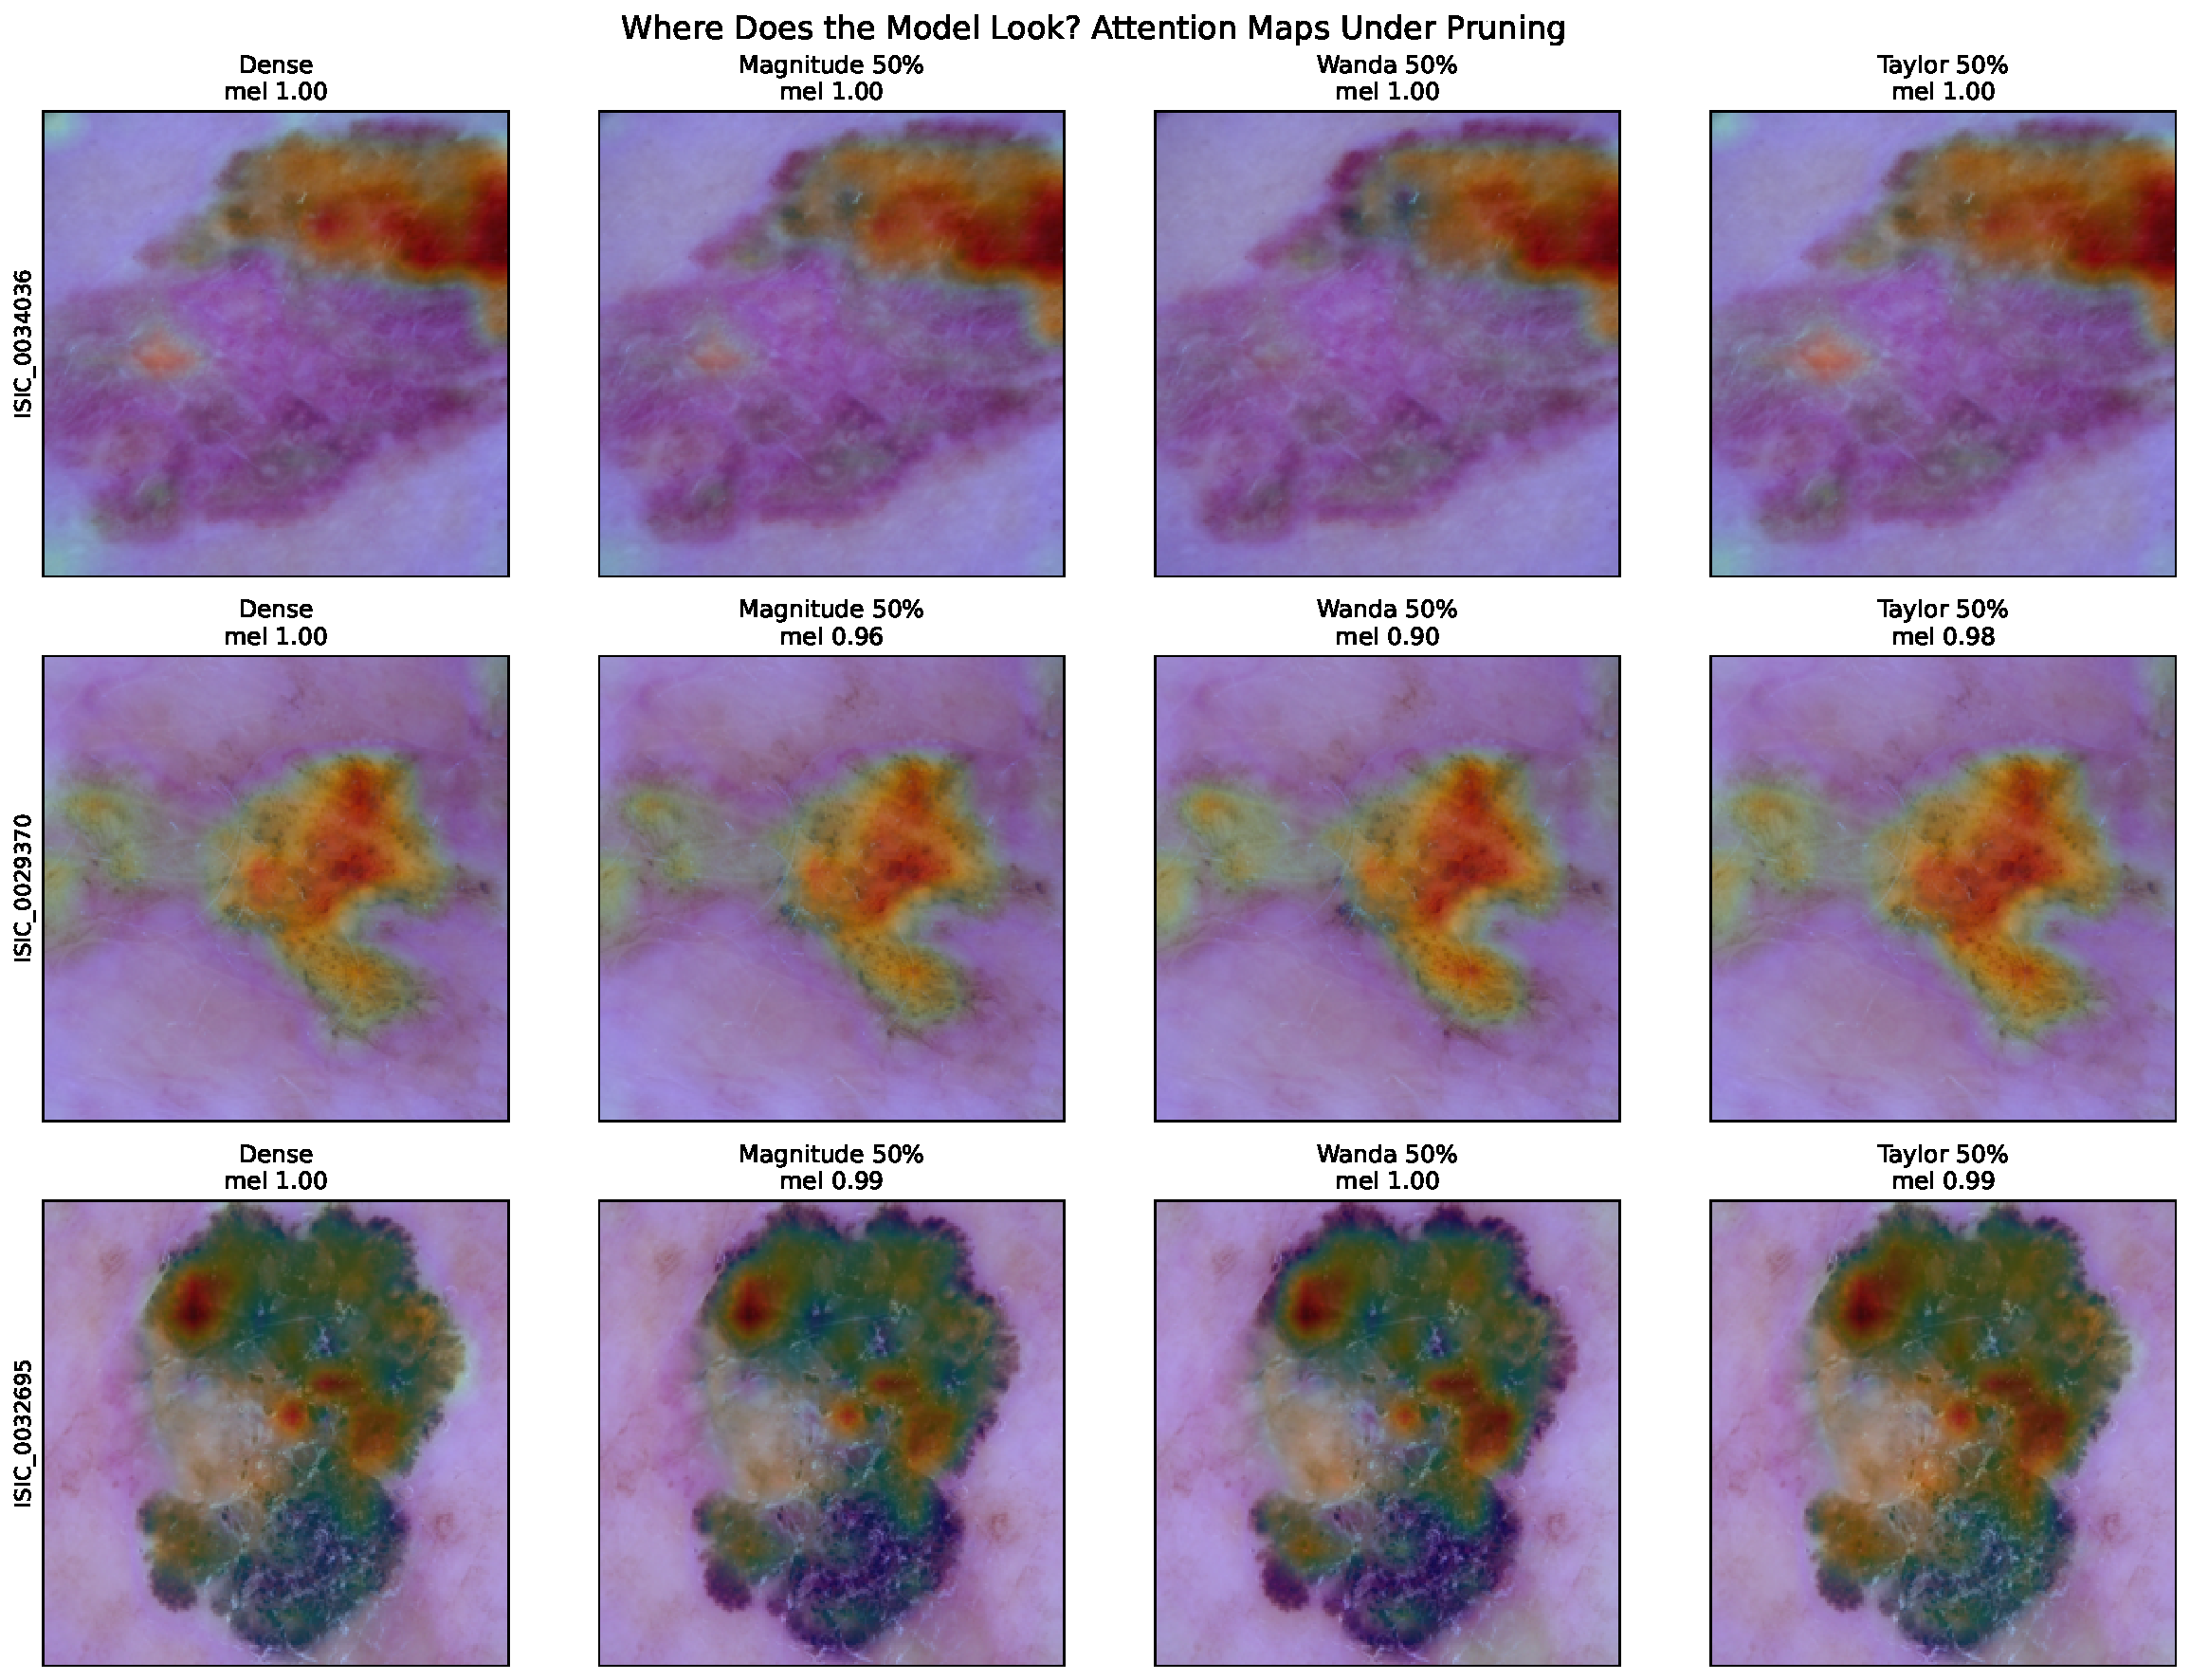
\includegraphics[width=\textwidth]{../results/figures_local/fig8_attention_maps.pdf}
\caption{Attention rollout for Dense, Magnitude 50\%, Wanda 50\%, and Taylor 50\%. The qualitative pattern agrees with Table~\ref{tab:attention}: Wanda still attends to the lesion region, and its problem lies in the downstream classifier.}
\label{fig:attention_maps}
\end{figure*}

This tells a biomedical team what to fix. If a compressed model fails because its attention misses the lesion, the fix is architectural or optimization-based. If the model still attends to the lesion but collapses at the classifier head, the fix is calibration-aware retraining or a different pruning criterion. Our results point to the second case.

\subsection{Sparsity placement and external baselines}
The local exploratory figures and the aggregated non-uniform table agree that where a model is pruned can matter more than the exact score used to rank weights. Sensitivity-guided non-uniform allocation can rescue Wanda, but not every policy helps. The best Wanda rescue comes from the more aggressive binned\_k5 setting rather than the default binned policy: it reaches a balanced accuracy of $0.857$ and a melanoma sensitivity of $0.741$. The learnable policy reaches $0.871$ balanced accuracy but with a higher \DCR{}. The continuous-temperature policies are less stable and are a poor first choice for a safe clinical default.

\begin{figure}[t]
\centering
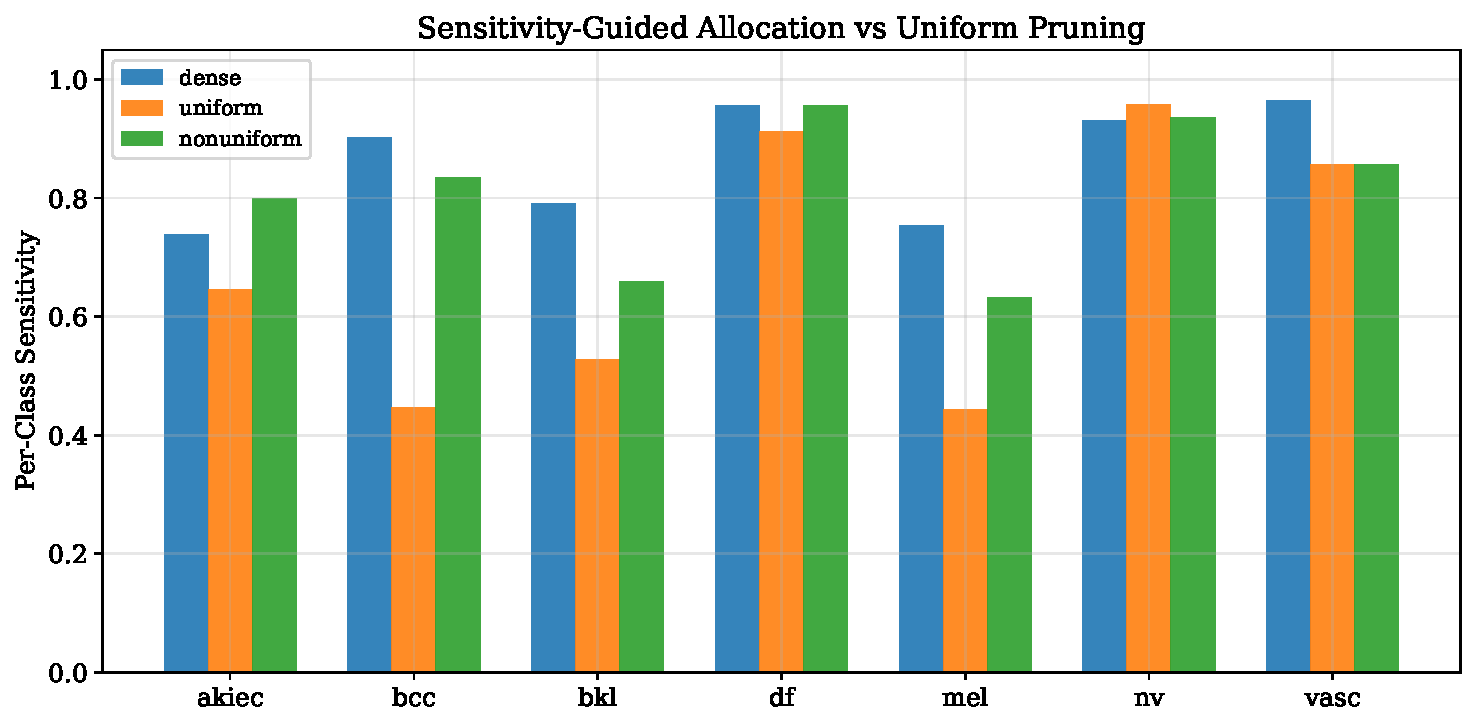
\includegraphics[width=\linewidth]{../results/figures_local/fig4_nonuniform_vs_uniform.pdf}
\caption{Sensitivity-guided non-uniform pruning from the exploratory run. For Wanda, redistributing sparsity by layer sensitivity restores a large fraction of the lost class recall. Magnitude gains much less from the same idea, which suggests the scoring rule and the sparsity allocation rule should be evaluated together.}
\label{fig:nonuniform}
\end{figure}

The external baselines leave the main ordering intact. Neither Paxton-style skewness pruning nor X-Pruner overturns the finding that Taylor is the best sparse default and that magnitude is not the safest choice for biomedical deployment. On balanced accuracy alone, X-Pruner is the strongest external 50\% baseline on DeiT-Small, but Taylor has the better combination of melanoma sensitivity and calibration. SparseGPT-pseudo is the worst fit for this medical task. The detailed non-uniform and baseline results are in the appendix; they are useful implementation guidance but are not the paper's main claim.

\subsection{Quantization, distillation, and deployment}
For deployment, start with INT8 quantization and then decide whether sparsity is necessary. Quantization shrinks the model without changing the structure of the learned function, which makes it the least risky compression stage. Pruning changes which learned connections survive, so the choice of pruning criterion matters.

Knowledge distillation does not provide robustness to pruning. On DeiT-Tiny (Table~\ref{tab:kd}), the distilled dense student has lower balanced accuracy than the directly fine-tuned one ($0.795$ vs.\ $0.865$), and after pruning the gap widens ($0.215$ vs.\ $0.353$), with worse melanoma AUROC and ECE.

Under the conservative clinical thresholds in the log companion files, every evaluated pipeline remains \texttt{academic\_only}. The experiments are strong enough to rank compression choices but not to claim unsupervised clinical readiness. On the same host, dense DeiT-Tiny runs at 11.61 ms on CPU and 2.57 ms on MPS, and dense DeiT-Small in the quantization run measures 20.3 ms mean latency and 22.0 ms at p95. These latencies are fast enough for interactive use, and they do not change the ranking that makes INT8 the safest first size reduction.

\begin{table*}[t]
\centering
\small
\caption{Selected deployment summary from the multi-seed personal quantization run. Quantization closely preserves dense behavior, but the pruning criterion still determines the downstream clinical tradeoff. We report size because it is the main deployment gain; latency depends on the backend and is discussed in the appendix.}
\label{tab:quant}
\resizebox{\textwidth}{!}{%
\begin{tabular}{lccccc}
\toprule
Configuration & Bal.\ Acc. & Mel.\ Sens. & Mel.\ AUROC & ECE & Size (MB) \\
\midrule
Dense                & $0.849 \pm 0.069$ & $0.864 \pm 0.077$ & $0.947 \pm 0.026$ & $0.038 \pm 0.015$ & $84.7$ \\
Quantized only       & $0.867 \pm 0.072$ & $0.890 \pm 0.077$ & $0.956 \pm 0.024$ & $0.031 \pm 0.017$ & $22.5$ \\
Magnitude 50\%       & $0.775 \pm 0.060$ & $0.585 \pm 0.057$ & $0.877 \pm 0.024$ & $0.038 \pm 0.006$ & $43.2$ \\
Magnitude 50\% + INT8 & $0.770 \pm 0.061$ & $0.611 \pm 0.073$ & $0.874 \pm 0.024$ & $0.038 \pm 0.008$ & $22.5$ \\
Wanda 50\%           & $0.602 \pm 0.011$ & $0.566 \pm 0.018$ & $0.845 \pm 0.013$ & $0.095 \pm 0.007$ & $43.2$ \\
Wanda 50\% + INT8    & $0.599 \pm 0.012$ & $0.555 \pm 0.023$ & $0.841 \pm 0.012$ & $0.090 \pm 0.007$ & $22.5$ \\
\bottomrule
\end{tabular}}
\end{table*}

For teams that need a smaller model quickly, Table~\ref{tab:quant} gives the practical answer. INT8 provides the large size reduction, Taylor remains the better sparse choice, and Wanda is acceptable only when recall is the overriding goal and calibration is re-checked afterwards.

\section{Discussion and Practical Guidance}
Biomedical compression should be judged by clinical behavior as well as aggregate accuracy. Our results lead to the following guidance.

\begin{itemize}[leftmargin=*,itemsep=2pt,topsep=2pt]
  \item Use lesion-grouped splits. Image-level splitting is too optimistic for dermoscopy because the same lesion can appear several times.
  \item Interpret balanced accuracy, melanoma AUROC, ECE, and \DCR{} together. Sensitivity alone is not enough.
  \item Start with INT8, then choose sparsity. Quantization is the lowest-risk compression stage, and if sparsity is required, Taylor is the safest default in this study.
  \item Use Wanda only with non-uniform sparsity. Non-uniform allocation can rescue it, but that makes it a recall-first option rather than a general improvement.
  \item Do not assume distillation fixes pruning. In our runs, the distilled student was worse than direct fine-tuning both before and after pruning.
  \item Validate on the target device. Measure latency, calibration, and operating points on the actual deployment runtime instead of inferring them from parameter count.
  \item Treat the current pipelines as research-only. Under the conservative clinical thresholds used here, every evaluated configuration remains \texttt{academic\_only}.
\end{itemize}

For biomedical integration, the recommendation is conservative but usable. If you can afford only one compression step, use INT8. If you need sparsity, use Taylor and validate the operating point that matters clinically. If Wanda looks attractive because it seems recall-friendly, check calibration and false positives before you ship.

\section{Limitations}
\begin{itemize}[leftmargin=*,itemsep=2pt,topsep=2pt]
  \item The core claim rests on one dataset and one imaging modality, so the HAM10000 results may not transfer to other settings.
  \item Some auxiliary experiments are exploratory follow-ups from the local run. They inform implementation choices, but the main pruning claim does not depend on them.
  \item The recovery and calibration follow-ups are not decisive, although they do show that the ranking barely changes under these extra settings.
  \item We do not test generalization to a second cohort; that would need a separate study.
\end{itemize}

\section{Conclusion}
Compression in biomedical vision affects safety as well as size. On HAM10000, the failure mode depends on how the model is compressed. Magnitude pruning is the least safe baseline. Wanda can look good on sensitivity while calibration and discrimination degrade. Taylor is the strongest sparse default in this study. INT8 quantization is the safest first compression stage, and the auxiliary experiments show that recovery, distillation, and calibration-size changes do not overturn the basic ranking.

The practical result is a deployment recipe rather than a new algorithm: use lesion-grouped splits, report clinical metrics together, start with INT8, and use Taylor when you need sparsity.

\appendix
\section{Layer-Wise Mechanism and Negative Results}
Figure~\ref{fig:perlayer} identifies the layers that matter most for diagnostic behavior. In the local exploratory run, the MLP blocks are the most damage-sensitive components and patch embedding is comparatively stable. This matches the intuition that the model's class-conditional behavior lives in the middle and late transformer blocks rather than in the first projection.

We also checked an activation-outlier hypothesis: that a simple relationship between heavy-tailed activation statistics and pruning damage could explain Wanda's behavior. The project summary reports near-zero correlations. This negative result rules out the most obvious explanation and keeps us from committing to a false mechanism.

\section{Non-Uniform Allocation and External Baselines}
Table~\ref{tab:nonuniform} shows the non-uniform allocation results from the multi-seed personal aggregate. Binned non-uniform sparsity can rescue Wanda, while a continuous-temperature rule is much less stable. A cleverer allocation policy does not always win; sparsity placement interacts with the pruning criterion.

\begin{table*}[t]
\centering
\small
\caption{Non-uniform allocation on DeiT-Small at 50\% average sparsity. The binned policy most clearly rescues Wanda; the continuous policy is less stable.}
\label{tab:nonuniform}
\resizebox{\textwidth}{!}{%
\begin{tabular}{lllccc}
\toprule
Criterion & Policy & Bal.\ Acc. & Mel.\ Sens. & Mel.\ AUROC & \DCR \\
\midrule
Magnitude & uniform         & $0.787 \pm 0.025$ & $0.569 \pm 0.053$ & $0.881 \pm 0.019$ & $1.87 \pm 0.42$ \\
Magnitude & binned\_default & $0.758 \pm 0.047$ & $0.452 \pm 0.064$ & $0.858 \pm 0.034$ & $2.50 \pm 0.87$ \\
Magnitude & continuous\_t1  & $0.652 \pm 0.120$ & $0.240 \pm 0.119$ & $0.793 \pm 0.047$ & $2.14 \pm 1.35$ \\
Wanda     & uniform         & $0.612 \pm 0.018$ & $0.539 \pm 0.041$ & $0.837 \pm 0.019$ & $0.77 \pm 0.09$ \\
Wanda     & binned\_default & $0.841 \pm 0.036$ & $0.727 \pm 0.068$ & $0.918 \pm 0.012$ & $2.62 \pm 0.61$ \\
Wanda     & continuous\_t1  & $0.755 \pm 0.075$ & $0.579 \pm 0.110$ & $0.891 \pm 0.045$ & $2.58 \pm 3.26$ \\
\bottomrule
\end{tabular}}
\end{table*}

The external baselines mainly serve as anchors for the main ranking. Paxton-style skewness pruning and X-Pruner are reasonable comparators, and neither overturns the result that Taylor is the strongest sparse default in this study.

\begin{table}[t]
\centering
\small
\caption{External pruning baselines on the multi-seed aggregate. These values anchor the comparison and do not change the main ranking.}
\label{tab:baselines}
\begin{tabular}{llccc}
\toprule
Model & Method & Bal.\ Acc. & Mel.\ Sens. & \DCR \\
\midrule
\multirow{3}{*}{DeiT-Small}
 & Paxton (50\%)  & 0.631 & 0.388 & 1.46 \\
 & X-Pruner (50\%) & 0.747 & 0.746 & 1.58 \\
 & SparseGPT (50\%) & 0.208 & 0.000 & 1.14 \\
\midrule
\multirow{3}{*}{DeiT-Tiny}
 & Paxton (50\%)  & 0.616 & 0.529 & 1.23 \\
 & X-Pruner (50\%) & 0.644 & 0.750 & 0.34 \\
 & SparseGPT (50\%) & 0.227 & 0.067 & 0.85 \\
\bottomrule
\end{tabular}
\end{table}

\section{Quantization, Distillation, and Edge Deployment}
INT8 closely preserves the dense model's clinical behavior while cutting size by roughly 3.8$\times$. The stacking results show that pruning, not quantization, causes most of the degradation, which makes quantization the safest first compression stage.

\begin{table*}[t]
\centering
\small
\caption{Selected quantization-stacking results from the personal multi-seed runs. Quantization is the safest size reduction, but pruning still controls the clinical tradeoff. Latency depends on the backend, so we do not base recommendations on it.}
\label{tab:stacking}
\resizebox{\textwidth}{!}{%
\begin{tabular}{lcccccc}
\toprule
Configuration & Bal.\ Acc. & Mel.\ Sens. & Mel.\ AUROC & Macro AUROC & ECE & Size (MB) \\
\midrule
Dense                & $0.849 \pm 0.069$ & $0.864 \pm 0.077$ & $0.947 \pm 0.026$ & $0.971 \pm 0.018$ & $0.038 \pm 0.015$ & $84.7$ \\
Quantized only       & $0.867 \pm 0.072$ & $0.890 \pm 0.077$ & $0.956 \pm 0.024$ & $0.977 \pm 0.016$ & $0.031 \pm 0.017$ & $22.5$ \\
Magnitude 50\%       & $0.775 \pm 0.060$ & $0.585 \pm 0.057$ & $0.877 \pm 0.024$ & $0.954 \pm 0.015$ & $0.038 \pm 0.006$ & $43.2$ \\
Magnitude 50\% + INT8 & $0.770 \pm 0.061$ & $0.611 \pm 0.073$ & $0.874 \pm 0.024$ & $0.953 \pm 0.016$ & $0.038 \pm 0.008$ & $22.5$ \\
Wanda 50\%           & $0.602 \pm 0.011$ & $0.566 \pm 0.018$ & $0.845 \pm 0.013$ & $0.918 \pm 0.009$ & $0.095 \pm 0.007$ & $43.2$ \\
Wanda 50\% + INT8    & $0.599 \pm 0.012$ & $0.555 \pm 0.023$ & $0.841 \pm 0.012$ & $0.917 \pm 0.009$ & $0.090 \pm 0.007$ & $22.5$ \\
\bottomrule
\end{tabular}}
\end{table*}

Figure~\ref{fig:stacking_perclass} shows the same result per class. The ``pruned only'' and ``pruned plus quantized'' bars are nearly identical for every class, and both differ substantially from the dense reference, so INT8 leaves the per-class sensitivity profile set by pruning essentially unchanged.

\begin{figure}[t]
\centering
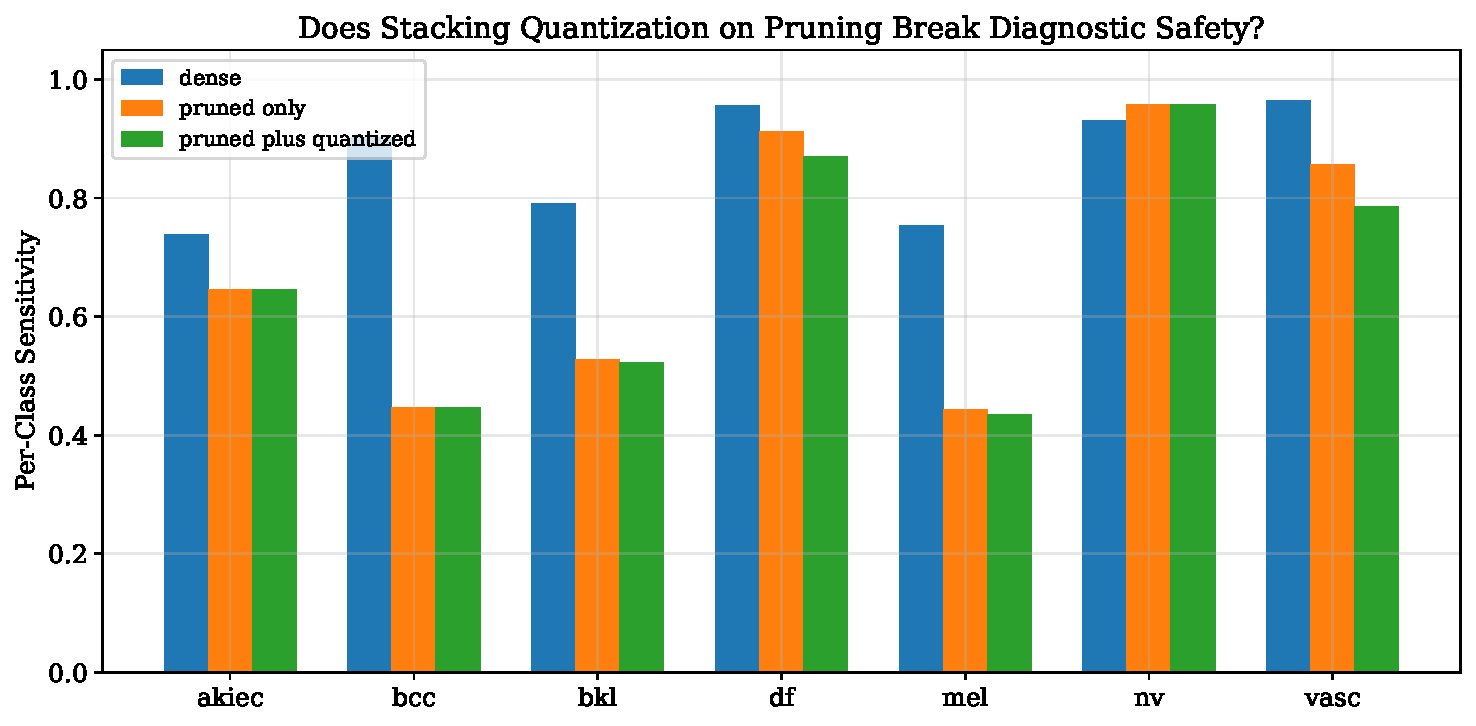
\includegraphics[width=\linewidth]{../results/figures_local/fig5_stacking.pdf}
\caption{Per-class sensitivity for dense, pruned, and pruned plus INT8 quantized DeiT-Small at 50\% magnitude sparsity. The pruned and pruned-plus-quantized bars track each other class by class, including on the dangerous classes (\akiec, \bcc, \mel). Pruning, not quantization, drives the clinical degradation.}
\label{fig:stacking_perclass}
\end{figure}

In the multi-seed personal runs, the distilled dense student scored below the directly fine-tuned dense model on balanced accuracy and melanoma AUROC, with similar ECE, and the distilled pruned student degraded further than the directly fine-tuned pruned one. In this setup, distillation is not a useful pre-treatment for sparsity.

\begin{table}[t]
\centering
\small
\caption{Knowledge distillation pre-treatment on DeiT-Tiny. Distillation does not add robustness; pruned distilled models remain fragile.}
\label{tab:kd}
\begin{tabular}{llccc}
\toprule
Variant & Pruned? & Bal.\ Acc. & Mel.\ AUROC & ECE \\
\midrule
Direct    & No  & $0.865 \pm 0.075$ & $0.947 \pm 0.027$ & $0.035 \pm 0.018$ \\
Distilled & No  & $0.795 \pm 0.023$ & $0.928 \pm 0.008$ & $0.033 \pm 0.009$ \\
Direct    & Yes & $0.353 \pm 0.019$ & $0.795 \pm 0.019$ & $0.120 \pm 0.014$ \\
Distilled & Yes & $0.215 \pm 0.029$ & $0.648 \pm 0.059$ & $0.161 \pm 0.032$ \\
Imagenet  & No  & $0.153 \pm 0.014$ & $0.524 \pm 0.072$ & $0.237 \pm 0.060$ \\
Imagenet  & Yes & $0.149 \pm 0.014$ & $0.577 \pm 0.107$ & $0.286 \pm 0.084$ \\
\bottomrule
\end{tabular}
\end{table}

Latency numbers are only reliable when measured on the actual target runtime. In the project logs, dense DeiT-Tiny ran at 11.61 ms on CPU and 2.57 ms on MPS on the same host. A biomedical deployment argument should rest on device-specific measurements like these.

\section{Recovery, Calibration, and the CNN Baseline}
Recovery fine-tuning mainly shows what does not rescue the model: in the multi-seed aggregate, the ranking stays largely unchanged across the sweep. The calibration-size ablation moves Wanda a little and leaves the overall recommendation unchanged.

\begin{table*}[t]
\centering
\small
\caption{Recovery sweep on the multi-seed aggregate. The sweep changes the numbers slightly but not the ordering.}
\label{tab:recovery}
\begin{tabular}{llcccc}
\toprule
Model & Criterion & Sparsity & Recovery epochs & Bal.\ Acc. & Mel.\ Sens. \\
\midrule
DeiT-Small & Magnitude & 50\% & 5/10/20 & $0.775 \pm 0.074$ & $0.585 \pm 0.070$ \\
DeiT-Small & Taylor    & 50\% & 5/10/20 & $0.746 \pm 0.060$ & $0.874 \pm 0.086$ \\
DeiT-Small & Wanda     & 50\% & 5/10/20 & $0.598 \pm 0.007$ & $0.533 \pm 0.019$ \\
DeiT-Tiny   & Magnitude & 50\% & 5/10/20 & $0.845 \pm 0.084$ & $0.789 \pm 0.059$ \\
DeiT-Tiny   & Taylor    & 50\% & 5/10/20 & $0.836 \pm 0.004$ & $0.700 \pm 0.035$ \\
DeiT-Tiny   & Wanda     & 50\% & 5/10/20 & $0.794 \pm 0.023$ & $0.717 \pm 0.020$ \\
\bottomrule
\end{tabular}
\end{table*}

\begin{figure}[t]
\centering
\includegraphics[width=\linewidth]{../results/figures_personal/fig7_recovery_balacc.pdf}
\includegraphics[width=\linewidth]{../results/figures_personal/fig7_recovery_mel.pdf}
\caption{Recovery fine-tuning on balanced accuracy and melanoma sensitivity. Recovery does not change the criterion ranking enough to alter the biomedical recommendation.}
\label{fig:recovery}
\end{figure}

\begin{table}[t]
\centering
\small
\caption{Calibration-size ablation for Wanda on the multi-seed aggregate. Larger calibration sets help only modestly and do not make Wanda a better sparse default than Taylor.}
\label{tab:calibration}
\begin{tabular}{ccc}
\toprule
Calibration size & Bal.\ Acc. & Mel.\ Sens. \\
\midrule
16  & 0.610 & 0.455 \\
32  & 0.611 & 0.375 \\
64  & 0.612 & 0.410 \\
128 & 0.619 & 0.407 \\
256 & 0.618 & 0.436 \\
512 & 0.611 & 0.408 \\
\bottomrule
\end{tabular}
\end{table}

The MobileNetV2 baseline is a sanity check showing that fragility under unstructured pruning is not unique to transformers. The CNN collapses faster than the ViTs under the same pruning settings. This makes the main recommendation more relevant, because the problem lies in the compression criterion and the deployment objective rather than in the architecture.

\begin{table}[t]
\centering
\small
\caption{MobileNetV2 baseline. This is an exploratory architecture check, not a generalization claim.}
\label{tab:mobilenet}
\begin{tabular}{lccc}
\toprule
Setup & Bal.\ Acc. & Mel.\ Sens. & Macro AUROC \\
\midrule
Dense      & 0.766 & 0.633 & 0.953 \\
Magnitude 30\% & 0.722 & 0.604 & 0.950 \\
Magnitude 50\% & 0.251 & 0.071 & 0.872 \\
Magnitude 70\% & 0.143 & 0.000 & 0.573 \\
Wanda 30\%     & 0.166 & 0.004 & 0.835 \\
Wanda 50\%     & 0.143 & 0.000 & 0.532 \\
Wanda 70\%     & 0.143 & 1.000 & 0.573 \\
\bottomrule
\end{tabular}
\end{table}

\clearpage
\bibliographystyle{plainnat}
\bibliography{references}

\end{document}
